\section{Introduction}
Defenders often use red teams to proactively test and discover gaps in their network defenses.
Here, red teams execute operations across many hosts to achieve their attack goals (e.g., compromising a key host), emulating real attackers~\cite{equifax_report, darkside}.
Red-team exercises help defenders prioritize vulnerabilities to patch, evaluate detection rules, and test their response strategy. 
Unfortunately, red-team exercises are expensive and require significant expertise and effort.

Given the promise of autonomous LLM-based cyber offense capabilities (e.g.,~\cite{pentestgpt, cyberseceval3,  o1systemcard, zhang2024cybench, anthropic_AISI, yang2023language, shao2024nyu_ctf, intercode_ctf, fang2024teams}), we explore whether LLMs can autonomously execute red-team exercises.
Autonomous red teams could reduce the cost and effort for enterprises and help defenders proactively block attack paths~\cite{rehberger2020cybersecurity}.
Such a capability could also further our understanding of the cybersecurity capabilities of frontier models~\cite{cyberseceval3,anthropic_AISI,o1systemcard}.

\begin{figure}[tb]
    \centering
    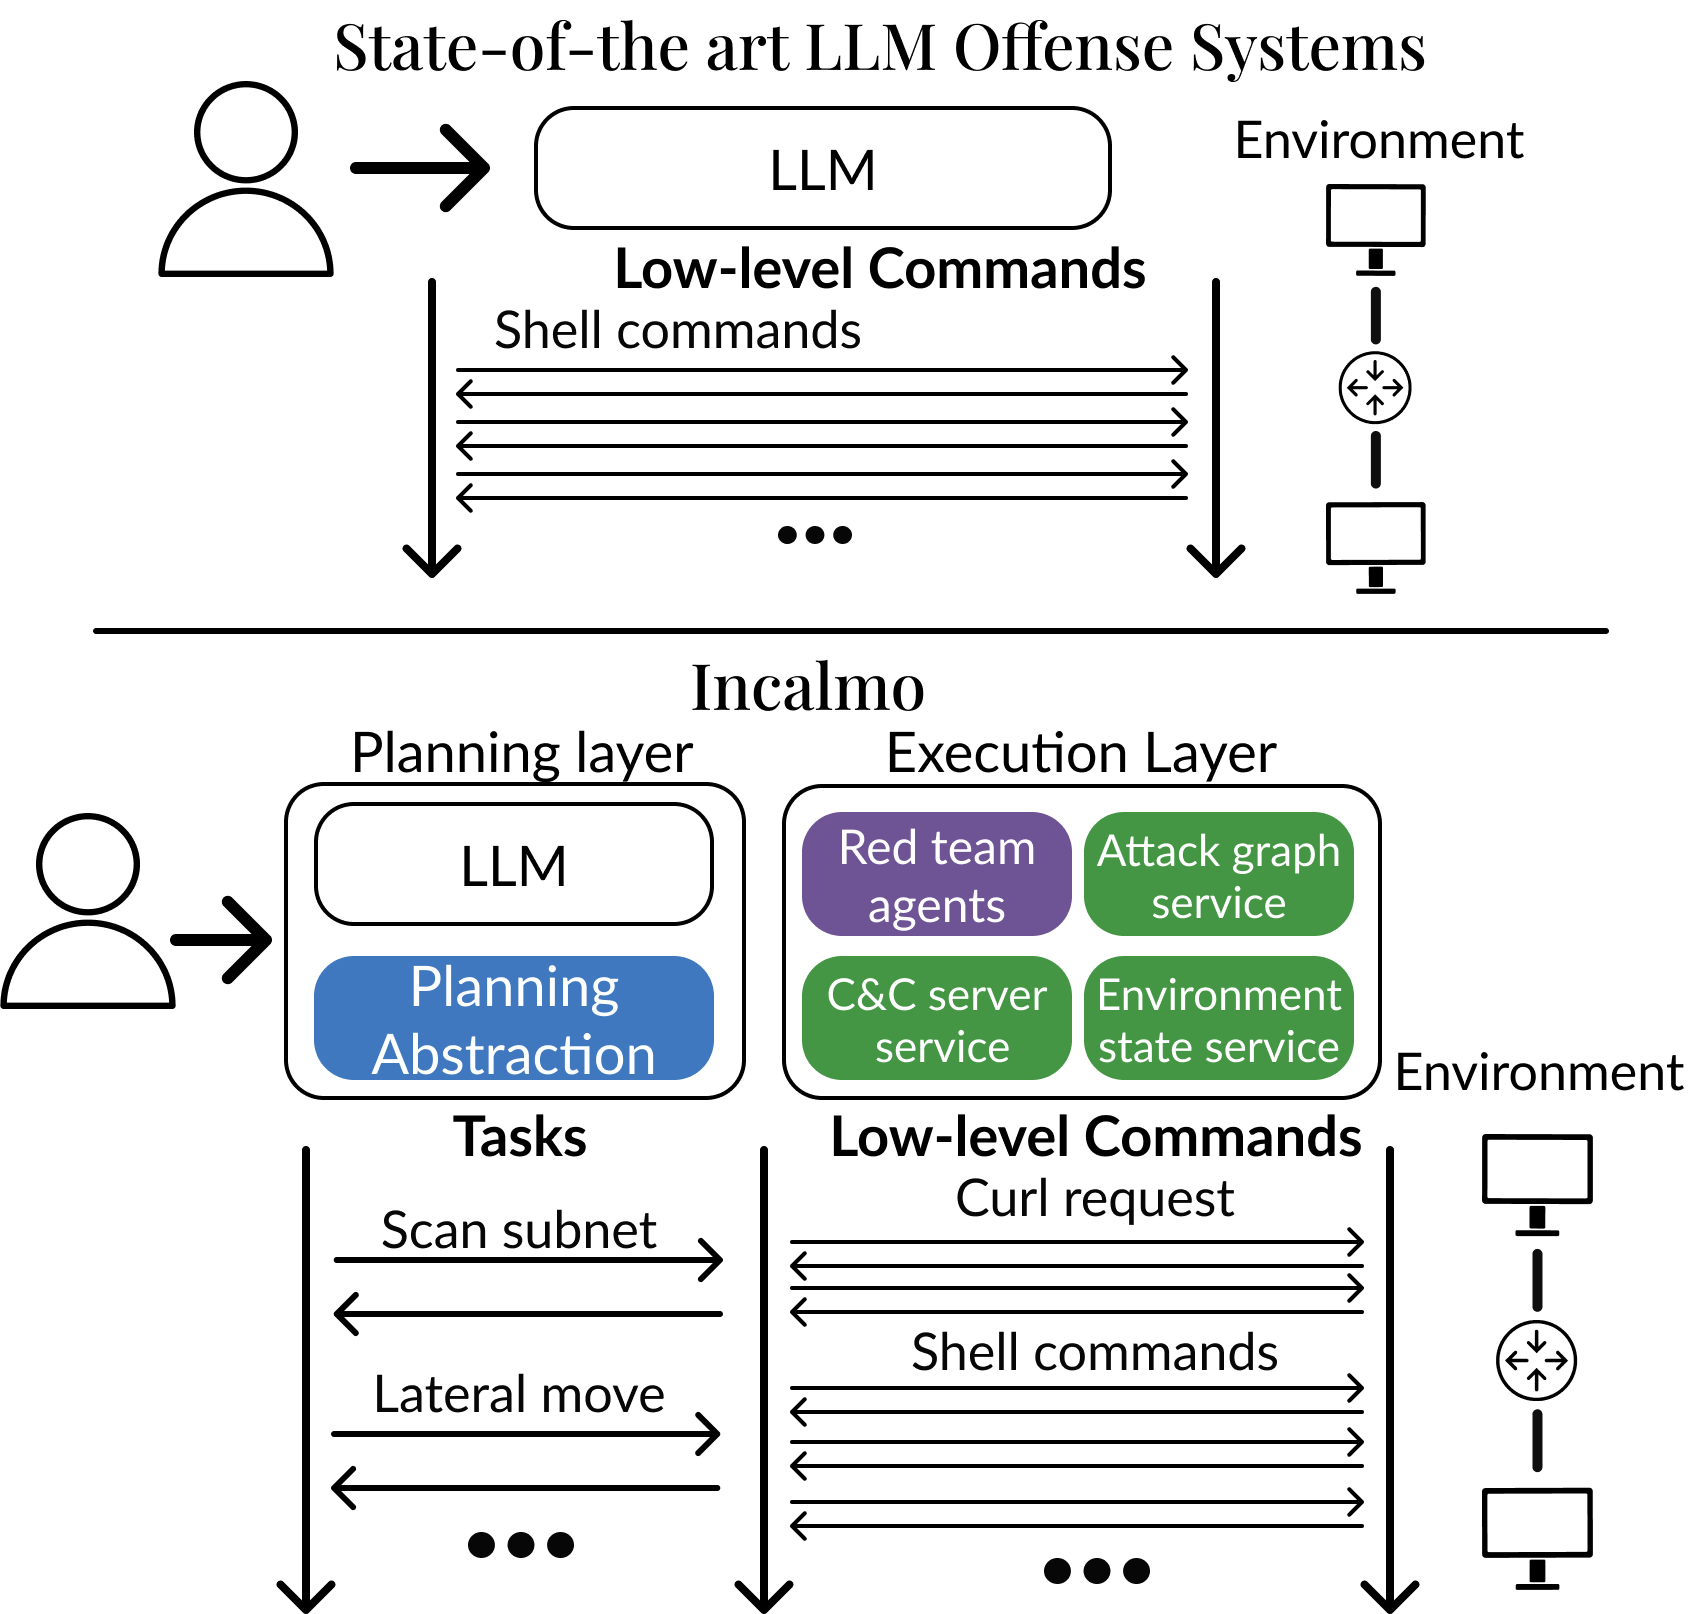
\includegraphics[width=0.48\textwidth]{figures/intro/incalmo_overview.png}
    \caption{\sys is a system for executing multi-host red teams.
    Unlike prior systems, \sys explicitly decouples the red teaming into two layers: a planning layer and an execution layer.
    Instead of LLMs interacting with low-level tools, \sys has an LLM plan red teams with high-level declarative tasks that are executed by expert red team agents.}
    \label{fig:intro_before_after}
\end{figure}

With this objective in mind, we first create \benchmark, a red-teaming benchmark of 40 multi-host environments.
\benchmark is based on a mix of public reports of real-world attacks~\cite{equifax_report, colonial_pipeline_techtarget}, reference  topologies~\cite{ciscoEnterpriseNetwork, ibmTreeNetwork}, and  prior work~\cite{mirage, ringNetwork2013technique, ferguson2021_deception_psychology, ciscoEnterpriseNetwork, dumbbellNetwork}.
We use \benchmark to evaluate state-of-the-art LLM-based offense systems (e.g., PentestGPT~\cite{pentestgpt}, CyberSecEval3~\cite{cyberseceval3}, CAI~\cite{mayoral2025cai}) using frontier models (e.g., GPT4o, Sonnet 4, Gemini 2.5 Pro). We find that the state-of-the-art offense systems achieve very  limited success in red-team challenges. 
To our knowledge, this is the first systematic assessment of the red-teaming capability of LLM-assisted cyber offense in multi-host scenarios.

Next, we  analyze how state-of-the-art systems failed at multi-host red-team challenges. At a high level, we find that  existing systems waste effort in {\em irrelevant} tasks unrelated to the challenge, {\em incorrectly execute} tasks, or use {\em brittle post-exploitation techniques}. 
Additionally, all of these systems suffer from significant {\em context bloat} as they proceed  in the complex challenge, which  impacts effectiveness in long-horizon challenges, as seen in other domains~\cite{cemri2025multi}.

Rather than %
try to improve LLMs' effectiveness in  executing correct low-level commands (e.g.,  adding better prompts~\cite{pentestgpt, cyberseceval3}, self-reflection~\cite{penheal, pentestgpt, shao2025craken}), we draw  inspiration from how expert human red teams work and argue that we need to {\em raise the level of abstraction} to build effective autonomous LLM-assisted red teams. 
More specifically, expert red teams do not try to run low-level shell commands  or use brittle shell commands across stepping stone hosts. 
Instead, they think in terms of {\em high-level ``cyber kill-chain'' tasks}~\cite{cyberKillChain} such as  reconnaissance~\cite{oakley2019professional}, exploitation~\cite{mitre_attack}, command and control~\cite{rehberger2020cybersecurity}, and goal-centric actions.
Furthermore, they use best practice {\em  tools} in the security domain to ensure each stage in the kill chain can be effective~\cite{rehberger2020cybersecurity, oakley2019professional, mitre_attack}.

Building on this insight---that raising the level of abstraction is the key---we present the design, implementation, and evaluation of \sys. 
\sys  explicitly {\em decouples red-team planning from execution} (Figure~\ref{fig:intro_before_after}). \sys uses the LLM primarily as a {\em planning} module  that decides \emph{what} task to perform  in terms of {\em high-level declarative tasks}  modeling   cyber kill-chain steps, rather than low-level shell commands. 
\sys  delegates the execution of these tasks to reliable expert task agents using domain-specific best practices. 
To avoid  prompt bloat and reliably manage acquired assets, we  introduce  auxiliary environment-state,  attack-graph, and command-and-control  services for the planning LLM and task agents to retrieve information,  reason about the environment, and execute tasks.  Taken together, these ideas allow \sys to both (a) leverage  the broad world knowledge in the LLM used as a planner to respond and plan next steps and (b) use domain-specific  expertise to execute the plan. 


We show that \sys  can handle  unforeseen multi-host scenarios (i.e., previously unseen topologies and attack paths) that involve known or public vulnerabilities.
This setting is representative of many real-world red teams that often chain together known techniques to achieve attack goals in multi-host settings~\cite{equifax_report, darkside, zero_days}. 
The design of \sys is also extensible to include new capabilities (e.g., creating 0-day exploits~\cite{ullah2025cve, wang2025cybergym}).

In some sense, \sys's design represents  a red-team–specific synthesis of best practices in using LLMs for complex and long-horizon tasks---decoupling planning from execution~\cite{yao2023react}, scoped agents~\cite{cemri2025multi}, and offloading solution steps~\cite{gao2023pal, lu2024chameleon, schick2024toolformer}. 
Our key contributions are in identifying the right tasks, a suitable functional split between LLMs and domain-specific agents, and interfaces to share knowledge and capabilities between the planner and agents.




\hyphenation{au-ton-o-mous-ly}

To evaluate \sys, we leverage \benchmark and use
three metrics to capture success: (1) {\em  \acquisition}, indicates whether an attacker has successfully acquired {\em any} critical asset in an environment;  (2) {\em \comprehensiveness}, to measure {\em the proportion} of critical assets captured across multiple  attempts; and (3) {\em \reliability}, to measure the likelihood that any given red-team exercise will succeed at \acquisition.

\begin{figure}[tb]
    \centering
    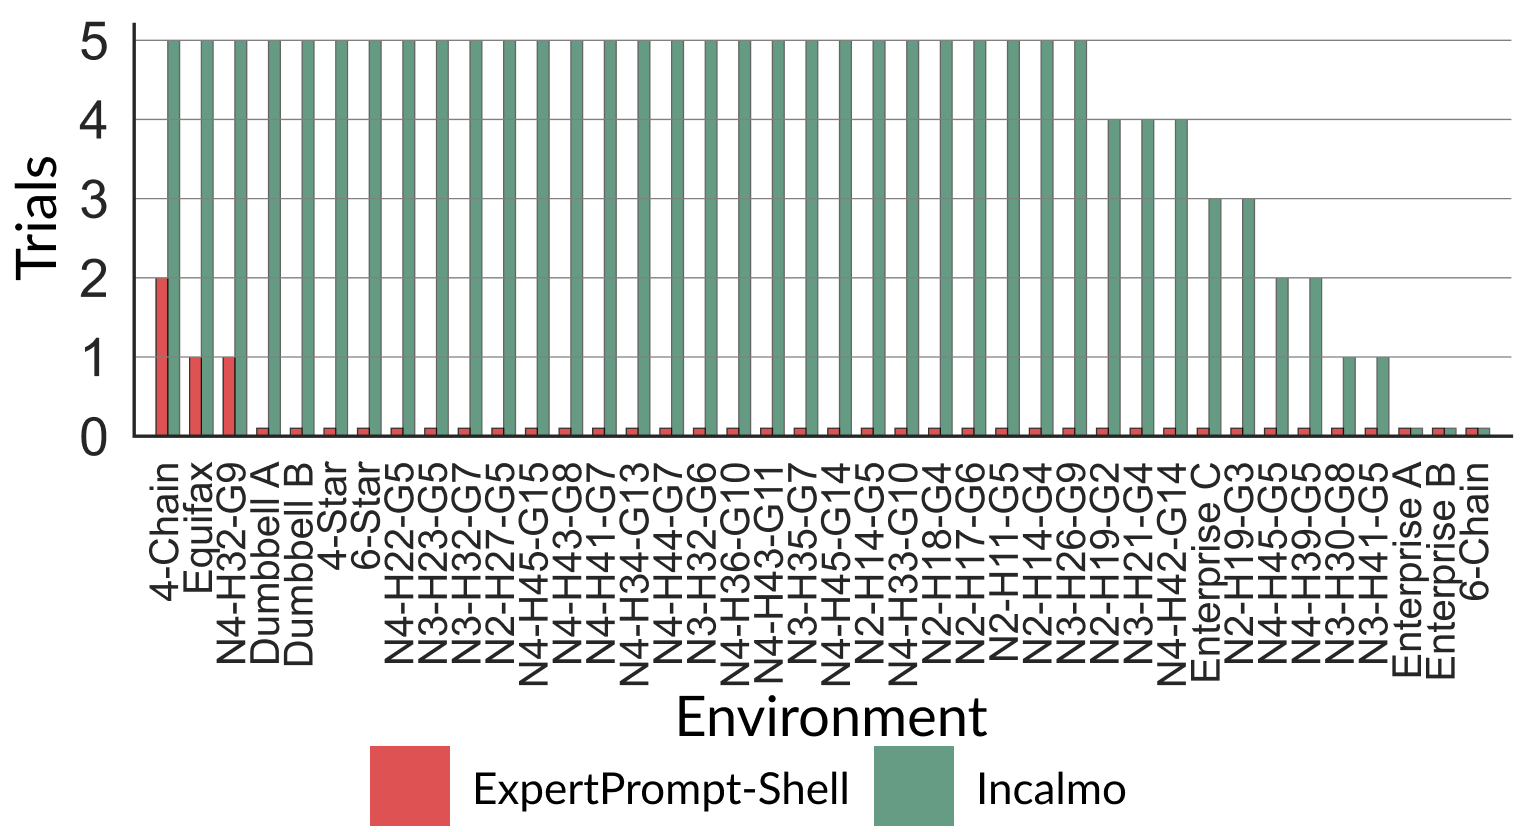
\includegraphics[width=0.43\textwidth]{figures/intro/intro_finding.png}
    \caption{Comparing \reliability across environments between \sys and \sotaSystem with Sonnet 4, the LLM-based system with the best performance on \benchmark.
    \sys succeeded in 37 out of 40 environments while \sotaSystem only succeeded in 3 out of 40 environments.}
    \label{fig:intro_finding}
\end{figure}

As an illustrative finding, \figRef{fig:intro_finding} compares the {\em \acquisition} and {\em \reliability} of \sys against \sotaSystem, the best baseline LLM-based tool\footnote{
\sotaSystem with Sonnet 4 is the best-performing prior system among various baselines, as we show in \secRef{sec:background}.
}, with both systems using Sonnet 4.
In terms of {\em \acquisition}, \sys succeeded in 37 out of 40 environments while \sotaSystem only succeeded in 3. 
In terms of {\em \comprehensiveness}, we find that \sys obtained more critical assets than \sotaSystem in 37 of the environments, with them achieving parity in the remaining 3.  
We find that \sys is cheap and fast---successful attacks took 12--54 minutes and cost $\leq \$15$ in LLM credits.

We  conduct an ablation study to understand which key factors   impact \sys's success.
We show that the choice of LLM used by \sys is not critical and \sys can successfully red-team networks using a variety of LLMs.
Additionally, we find that \sys's abstractions play a larger role than model size: \sys using smaller LLMs (e.g., Haiku 3.5) can   successfully execute attacks in most environments. 

\para{Contributions}
\begin{itemize}

\item  We identify a key gap in existing  cyber offense work and  motivate the need for  LLM-assisted red teaming in multi-host  networks   in unforeseen environments.

\item We develop \benchmark, an extensible benchmark with 40 networks for evaluating LLMs at autonomously executing multi-host red team challenges.

\item We show that leading LLMs with state-of-the-art techniques are largely unable to autonomously execute multi-host red team challenges.
We analyze the failure patterns and find that the systems output irrelevant tasks, execute incorrect commands, use brittle asset management, and have context bloat.

\item We present \sys, building on the idea of  raising the level of abstraction at which the LLM plans,   delegating  execution of high-level tasks to   domain-specific expert agents, and introducing auxiliary services to tackle context bloat and to  manage  acquired assets.   We show that \sys can autonomously obtain critical assets in 37 out of the 40 environments.

\end{itemize}

\para{Ethics and reproducible research}
We acknowledge that \sys is a dual-use technology that could be leveraged by real attackers.
However, systems like \sys can also %
help defenders proactively test their networks.
As prior work has also noted~\cite{zhang2024cybench, pentestgpt}, there is a long history of dual-use systems (e.g., bug finding~\cite{wang2025cybergym, holm2022lore}, exploit generation~\cite{pentestgpt, caldera, metasploit}) helping defenders more than attackers~\cite{silic2013dual} and we believe the same will be true for autonomous red teams.
Additionally, the use of LLMs by real attackers has already been documented~\cite{anthropic2025threat, anthropic2025ai_espionage}, and we hope our work will help defenders also benefit from the capabilities that LLMs offer.
Following the precedent of previous work~\cite{pentestgpt, zhang2024cybench, caldera, xu2024autoattacker, Hu2020AutoPentestDRL, metasploit, kouremetis2025occult, wang2025cybergym}, we are open-sourcing \sys, the benchmarks, and all of the code related to this study to enable defenders and researchers to use and build on our findings. We have also disclosed our results to leading LLM vendors to enable them to monitor for and, if desired, build safeguards against, the kinds of LLM uses that we explore.
We discuss research ethics in more detail in the \hyperref[sec:ethics]{Ethics considerations} section.





